)
\documentclass[a4paper, 11pt, notitlepage, english]{article}

\usepackage{babel}
\usepackage[utf8]{inputenc}
\usepackage[T1]{fontenc, url}
\usepackage{textcomp}
\usepackage{amsmath, amssymb}
\usepackage{amsbsy, amsfonts}
\usepackage{graphicx, color}
\usepackage{parskip}
\usepackage{framed}
\usepackage{amsmath}
\usepackage{xcolor}
\usepackage{multicol}
\usepackage{url}
\usepackage{flafter}
\usepackage{caption}

%\DeclareCaptionLabelSeparator{colon}{. }
\renewcommand{\captionfont}{\sffamily}
\renewcommand{\captionlabelfont}{\bf\sffamily}
\setlength{\captionmargin}{20pt}

\usepackage{geometry}
\geometry{headheight=0.01mm}
\geometry{top=24mm, bottom=29mm, left=39mm, right=39mm}

\renewcommand{\arraystretch}{1.2}
\setlength{\tabcolsep}{10pt}
\makeatletter
\renewcommand*\env@matrix[1][*\c@MaxMatrixCols c]{%
  \hskip -\arraycolsep
  \let\@ifnextchar\new@ifnextchar
  \array{#1}}
%
% Parametere for inkludering av kode fra fil
%
\usepackage{listings}

\DeclareMathAlphabet{\mathbfit}{OML}{cmm}{b}{it}

\definecolor{javared}{rgb}{0.6,0,0} % for strings
\definecolor{javagreen}{rgb}{0.25,0.5,0.35} % comments
\definecolor{javapurple}{rgb}{0.5,0,0.35} % keywords
\definecolor{javadocblue}{rgb}{0.25,0.35,0.75} % javadoc

\lstset{language=python,
basicstyle=\ttfamily\scriptsize,
keywordstyle=\color{javapurple},%\bfseries,
stringstyle=\color{javared},
commentstyle=\color{javagreen},
morecomment=[s][\color{javadocblue}]{/**}{*/},
% numbers=left,
% numberstyle=\tiny\color{black},
stepnumber=2,
numbersep=10pt,
tabsize=4,
showspaces=false,
captionpos=b,
showstringspaces=false,
frame= single,
breaklines=true}
%
% Definering av egne kommandoer og miljøer
%

\newcommand{\bt}[1]{\boldsymbol{#1}}
\newcommand{\mat}[1]{\textsf{\textbf{#1}}}
\newcommand{\I}{\boldsymbol{\mathcal{I}}}
\newcommand{\p}{\partial}
\renewcommand{\d}{\text{d}}
%
% Navn og tittel
%
\author{Jonas van den Brink \\ \texttt{j.v.d.brink@fys.uio.no}}
\title{Introduksjon til vitenskapelig programmering \\ Uke 4 \\ Sandvika vgs}

\begin{document}
\maketitle

Sist uke laget vi et program som løste bevegelsesligningene for fallskjermhopping. Vi startet med Newtons 2.\ lov, og så på kreftene som virket. Fra dette fant vi et uttrykk for akselerasjonen, og vi brukte så bevegelsesligningene vi vent gjelder ved konstant akselerasjon til å løse for hastigheten små steg fremover i tid.

Idag skal vi gjøre det samme for posisjon, og vi skal da se på strikkhopp som et eksempel. Når vi ser på strikkhopp, er det egentlig bare uttrykket for akselerasjon som endrer seg, alt annet kan være helt likt. Men ettersom at kreftene som virker på en strikkhopper avhenger av posisjonen til hopperen, må vi også løse for posisjonen.

Etter vi har sett på det kommer vi til å plott $g$-kreftene både for fallskjerm- og strikkhopperen. Vi kan da sammenligne strikk og fallskjermhopp baser på $g$-kreftene hopperen føler. Vi kommer også til å se på hvordan fallskjermen løses ut, og hvordan det påvirker $g$-kreftene hopperen utsettes for.

\clearpage

\section*{Å løse for posisjon}
Sist uke fant vi først et uttrykk for akselerasjonen for en fallskjermhopper som var
$$a(v) = g - \frac{1}{2}C\rho A v^2.$$
og vi brukte så bevegelsesligningene som gjelder ved konstant akselerasjon
$$v = v_0 + a t,$$
til å ta små "tidssteg" på $\Delta t$, som ga oss
\begin{align*}
v_1 &= v_0 + a(v_0)\Delta t \\  
v_2 &= v_1 + a(v_1)\Delta t \\
v_3 &= v_2 + a(v_2)\Delta t \\
&\hdots \\
v_{i+1} &= v_i + a(v_i)\Delta t.
\end{align*}

Vi har også en bevegelsesligning ved konstant akselerasjon som gjelder for posisjon
$$x = x_0 + v_0 t + \frac{1}{2}at^2,$$
vi kan bruke denne til å ta "tidssteg" på samme måte som for hastigheten
\begin{align*}
x_1 &= x_0  + v_0 \Delta t + \frac{1}{2} a(v_0) \Delta t^2 \\  
x_2 &= x_1  + v_1 \Delta t + \frac{1}{2} a(v_1) \Delta t^2 \\  
x_3 &= x_2  + v_2 \Delta t + \frac{1}{2} a(v_2) \Delta t^2 \\  
&\hdots \\
x_{i+1} &= x_i + v_i\Delta t + \frac{1}{2} a(v_i)\Delta t^2.
\end{align*}

\clearpage

\section*{Strikkhopp}
La oss nå se på en strikkhopper og kreftene som virker på henne. Vi kan tenke på strikken som en slags fjær når den er strukket ut. Men når strikken er "trykket" sammen gir den ingen kraft (i motsetning til en fjær, som virker "begge veier"). Når hopperen hopper fra toppen av en bru, er strikken slynget sammen, og kommer derfor ikke til å påvirke hopperen før hun har falt langt nok til at strikken begynner å bli strukket ut.  Vi kaller punktet der strikken akkurat ikke er begynnt å bli strukket ut for likevektspunktet.

La oss nå lage et referansesystem som passer bra til problemet vi ser på. Vi plasserer $x=0$ i likevektspunktet. Vi sier at strikken er 20 meter lang, så hopperen hopper fra et punkt som er 20 meter høyere enn likevektspunktet, altså i $x_0 = 20$ m. La oss også si at det går en elv under brua, og at brua er 60 m over elva.

\begin{figure}[h!b]
\centering
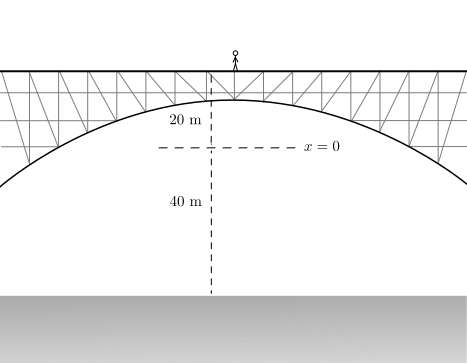
\includegraphics[width=0.9\textwidth]{Bungee_bridge}
\end{figure}

Vi ser nå at dersom posisjonen til hopperen er over likevektspunktet, så vil strikken ikke være strukket ut, og den virker ikke med noen kraft på hopperen. Siden vi har plassert likevektspunktet i $x=0$, betyr dette at strikkraften, som vi vil kalle $S$, er 0 hvis $x>0$.

Hvis $x<0$ derimot, ser vi at strikken er strukket ut, og vil dermed trekke hopperen oppover med en fjærkraft. Denne fjærkraften modellerer vi med det som kalles Hooke's lov, som sier at kraften fra en fjær som er strukket ut en lengde $x$ er gitt ved:
$$F = -kx,$$
der $k$ er fjærstivheten. 

Vi kan altså uttrykke den kraften fra strikken som en funksjon av posisjonen $x$ som følger:
$$S(x) = \begin{cases} 0 & \mbox{hvis } x>0 \\
-kx & \mbox{hvis } x \leq 0
\end{cases}.$$

I tilegg til snorkraften $S(x)$, virker det en tyngdekraft $mg$, og en luftmotstand $Dv$, på hopperen. Fra Newtons 2.\ lov
$$\sum F = ma,$$
har vi da
$$S(x) - mg - Dv = ma.$$
Vi løser for akselerasjonen, som vi nå ser er en funksjon av både posisjon og hastighet:
$$a(x,v) = \frac{S(x)}{m} - g - \frac{D}{m}v.$$

Ettersom at akselerasjon nå er en funksjon av både hastighet og posisjon, må vi løse for hastighet og posisjon samtidig, så vi har
\begin{align*}
v_1 &= v_0 + a(x_0, v_0)\Delta t \\
x_1 &= x_0 + v_0\Delta t + \frac{1}{2}a(x_0, v_0)\Delta t^2 \\
v_2 &= v_1 + a(x_1, v_1)\Delta t \\
x_2 &= x_1 + v_1\Delta t + \frac{1}{2}a(x_1, v_1)\Delta t^2 \\
&\hdots \\
v_{i+1} &= v_i + a(x_i, v_i)\Delta t \\
x_{i+1} &= x_i + v_i\Delta t + \frac{1}{2}a(x_i, v_i)\Delta t^2 \\
\end{align*}

\clearpage

\section*{Kode strikkhopp}
Du skal nå endre programmet du skrev sist uke til å løse for strikkhopping. Her er malen på hva programmet skal inneholde
\begin{enumerate}
    \item Importer pylab, det er alt vi kommer til å trenge.
    \item Skriv inn alle parameterene vi trenger. Bruk $m=60$, $v_0=0$, $x_0=20$, $D=10$. Gjett på en verdi for fjærstivheten $k$, vi kommer til å justere den etterhvert.
    \item Definer snorkraften $S(x)$. Her må du bruke \verb+def+ til å definere en funksjon, og en \verb+if+-test inne i funksjonen for å sjekke om $x>0$ eller $x<=0$. 
    \item Definer akselerasjonen som funksjon av både posisjon og hastighet. \verb+def a(x,v):+.
    \item Definer $\Delta t = 0.01$ (Hint: kall variablen \verb+dt+ i programmet ditt), $T=60$ og $n = T/dt$
    \item Opprett tre \emph{arrays}, ett for hastigheten $v$, ett for posisjonen $x$ og ett for tiden $t$. Vi vil at de skal være tomme, og ha plass til $n+1$ elementer, så bruk \verb+zeros+ kommandoen. 
    \item Sett første element i $x$-arrayet til å være $x_0$. Altså \verb+x[0] = x0+.
    \item Lag en \verb+for+-løkke som går over $i=0,1,2,\ldots,n$. (Hint, bruk \verb+range+.)
    \item Inne i løkka, regn ut $t[i+1]$, $v[i+1]$ og $x[i+1]$. Fra de følgende formlene
    \begin{align*}
    t_{i+1} &= t_i + \Delta t, \\
    v_{i+1} &= v_i + a(x_i, v_i)\Delta t, \\
    x_{i+1} &= x_i + v_i\Delta t + \frac{1}{2}a(x_i, v_i)\Delta t^2.
    \end{align*}
    Vi har altså
    \begin{lstlisting}
for i in range(n):
    t[i+1] = t[i] + ...
    v[i+1] = v[i] + ...
    x[i+1] = x[i] + ...    
    \end{lstlisting}
    \item Plot resultatet for å sjekke at alt har blitt gjort riktig (Hint: \verb+plot(t,x)+).
\end{enumerate}

\subsection*{Oppgave}
\begin{itemize}
    \item[a)] Pynt på plottet ditt. Sett navn på akser osv.
    \item[b)] Ved å se på plottet, prøv å juster fjærstivheten $k$ sånn at hopperen akkurat rører vannet. Altså at bunnen av kurven akkurat når $-40.$
    \item[c)] Skriv ut makshastigheten hopperen opplever. Hint: \verb+max(v)+. Hvordan er dette sammenlignet med makshastigheten til fallskjermhopperen?
\end{itemize}

\clearpage

\section*{Plotte $g$-krefter}
Begrepet $g$-kraft er noe misvisende, da det egentlig ikke er snakk om "krefter" man opplever - men akselerasjon. Når menneskekroppen blir akselerert, føler vi dette som vekt. Tenkt for eksempel når du sitter i en bil som kjører gjennom en sving, og du blir "dratt" til siden. Disse akselerasjonene føles altså ut som en slags kraft på kroppen, og det er derfor vi snakket om $g$-krefter. Bokstaven "g" i $g$-kraft står for gravitasjon, og det er fordi vi sammenligner den kraften en person med tyngdekraften. Når du står helt i ro, føler du $1g$ fra tyngdekraften. I en berg-og-dalbane vil man etterhvert som man følger banen oppleve mye forskjellige $g$-krefter etterhvert som man akselerer inn og ut av svinger og opp og ned bakker. Når vi har et hurtig dykk nedover på en berg-og-dalbane blir man vektløs, som altså er $0g$, eller fritt fall. En fordel med å snakke om $g$-krefter fremfor de faktiske fysiske kreftene som virker på et objekt, er at de ikke avhenger av massen. Alle personer vil altså kjenne de samme $g$-kreftene i den samme berg-og-dalbanen.

For å regne ut $g$-kreftene hopperen føler i begge tilfeller trenger vi egentlig bare å legge til et nytt array i løkka, hvor vi regner ut akselerasjonen som virker på hopperen, deler på $g$ og legger til 1. Koden er som følger:
\begin{lstlisting}
gforces = zeros(N+1)
...


for i in range(N):
    t[i+1] = t[i] + ...
    v[i+1] = v[i] + ...
    x[i+1] = x[i] + ...
    gforces[i] = a(x[i],v[i])/g + 1
\end{lstlisting}

\subsection*{Oppgave}
Regn ut og plot $g$-kreftene som virker på både fallskjerm- og strikkhopperen i programmet ditt. Sammenlign plottene, er de forskjellige? Forklar så godt du kan hvorfor de to er forskjellige.

\clearpage

\section*{Utløse fallskjermen}
Vi har nå kommet til tidspunktet der vi skal løse ut fallskjermen i programmet vårt. Vi har nevnt tidligere at det eneste vi egentlig trenger å gjøre er å endre luftmotstandskoeffisienten $C$ til $C_{\rm P} = 1.8$ og frontarealet $A$ til $A_{\rm p} = 44$. Vi har hitill simulert fallskjerm hopperen i $T=60$ sekunder, la oss øke denne tiden til 180 sekunder. Men vi lar fortsatt den første løkka bare gå over de første 60 sekundene, deretter endrer vi $C$ og $A$, og løser for de siste 120 sekundene, altså
\begin{lstlisting}
dt = 0.01
T = 180
n = int(T/dt)

# Simuler de forste 60 sekundene
for i in range(0, 60/dt):
    t[i+1] = t[i] + dt
    v[i+1] = v[i] + a(v[i])*dt
    gforces[i] = 1 - a(v[i])/g

# Endre C og A
C = C_p
A = A_p

# Simuler de siste 120 sekundene
for i in range(60/dt, 180/dt):
    t[i+1] = t[i] + dt
    v[i+1] = v[i] + a(v[i])*dt
    gforces[i] = 1 - a(v[i])/g
\end{lstlisting}

Nå kan vi plotte både hastigheten mot tid, og $g$-kreftene. Hva ser vi da? Et problem vi har fått er at vi endrer verdiene av $C$ og $A$ altfor brått. Dette er altså som om fallskjermen hadde blitt utløst umiddelbart, som hadde bremset ned hopperen enorm fort, og fører til nesten 100 $g$! Alt over 10 $g$ kan være livsfarlig og de fleste vanlige personer begynner å besvime når man går over $5$g.

Moderne fallskjermer er defor laget for å løse seg ut saktere med vilje, det gir dermed en roligere nedbremsning. La oss prøve å simulere at fallskjermen bruker 5 sekunder på å løse seg fullstendig ut, og se hvordan de påvirker $g$-kreftene. Vi lager nå tre løkker. En helt uten skjerm, en der fallskjermen er i prosessen å løse seg ut, og en der skjermen er helt løst ut.

\begin{lstlisting}
dt = 0.01
T = 180
n = int(T/dt)

# Simuler de forste 60 sekundene
for i in range(0, 60/dt):
    t[i+1] = t[i] + dt
    v[i+1] = v[i] + a(v[i])*dt
    gforces[i] = 1 - a(v[i])/g

# Simulerer de neste 5 sekundene
for i in range(60/dt, 65/dt):
    C += (C_p-C)/(5/dt)
    A += (A_p-A)/(5/dt)

    t[i+1] = t[i] + dt
    v[i+1] = v[i] + a(v[i])*dt
    gforces[i] = 1 - a(v[i])/g

# Simuler de siste 115 sekundene
for i in range(65/dt, 180/dt):
    t[i+1] = t[i] + dt
    v[i+1] = v[i] + a(v[i])*dt
    gforces[i] = 1 - a(v[i])/g
\end{lstlisting}


\end{document}
